\section{\acrlong{pid} Controller}
\label{ss:pid}
The motors used with the \gls{nxt} are assumed to be cheap in the sense there is no guarantee that an instruction is carried out as precisely as specified. For example, it cannot be assumed that two of the same motors will yield an identical result when instructed to run for a given time frame. The motors are \glspl{dcm}, so it is not possible to instruct them to turn a certain amount of degrees.
To regulate and make sure the motors controlling the targeting device are responsive, as well as carry out the instructions given as precise as possible, it has been chosen to use a \gls{pid} controller. This controller is essentially an algorithm which takes feedback into consideration and compensates for it. It regulates the power at which the motor is working, increasing the power when the motor is far away from its target, and decreasing the power as it approaches the desired angle.  
The mathematical formula for this controller is as follows \citep{pid_controller}:

\begin{equation} \label{pid_formula}
[PID-controller] \
u(t) = K_p *e(t) + K_i \int_0^t e(\tau)d\tau + K_d*
\frac{de}
     {dt}
\end{equation}
There are several adjustable constants denoted by $K$. The algorithm consists of three terms. The first term, $K_p*e(t)$ is a constant multiplied by a tracking error, which is the running difference between the desired input value and the current actual value. The second term, $K_i \int_0^t e(\tau)d\tau$, is a constant multiplied by the running summation of errors. The third term, $K_d* \frac{de}{dt}$, is the last constant multiplied by the difference between the current error and the previous error from last iteration. $dt$ is the interval at which the function is executed in milliseconds, and can be integrated into the three adjustable constants when the controller has a well-defined, confined purpose.

The adjustable parameters all have a specific influence on the controller, as can be seen in table \ref{pid_char}. There are four factors that to some extent are influenced by each of the parameters. Rise time is the time it takes to reach the desired value. Overshoot encodes the degrees of overshoot on the first rise. Settling time is the time it takes to settle itself within a certain range of the desired value. S-S error is short for steady-state error, and is responsible for the difference between the actual final value and the desired value.
These factors are illustrated on the graph shown on \ref{fig:pid_graph} with example values for the parameters.
\begin{table}[H]
\begin{tabular}{|l|l|l|l|l|}
\hline
RESPONSE & RISE TIME    & OVERSHOOT & SETTLING TIME & S-S ERROR \\ \hline
Kp          & Decrease     & Increase  & Small Decrease  & Decrease  \\ \hline
Ki          & Decrease     & Increase  & Increase      & Eliminate \\ \hline
Kd          & Small Increase & Decrease  & Decrease      & No Change \\ \hline
\end{tabular}
\caption{Table showing parameter influence based on \citep[University of Michigan]{pid_controller}}
\label{pid_char}
\end{table}

\begin{figure}[H]
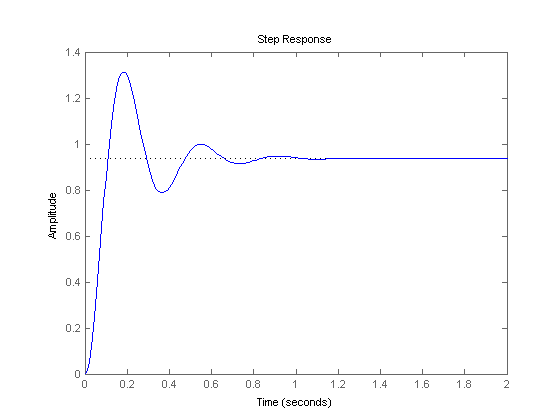
\includegraphics[scale=1]{graphics/pid_graph.png}
\caption{Example graph of a \gls{pid} controllers effect over time with example constant values\cite{pid_controlle_picr}}
\label{fig:pid_graph}
\end{figure}
Using the graph seen on \ref{fig:pid_graph} as an example, the rise time is approximately 0.1 sec, overshoot is 0.3 amplitude, settling time is around 1 second with very little error, and the steady-state error is approximately 0 amplitude. The constants can be fine-tuned to reduce and eliminate these factors.

To be able to adapt the \gls{pid} controller to the \gls{nxt} motors it will be necessary to customize different values for the two motors, as they operate under different loads. The three parameter values are easily found from similar projects, however the different weights on the motors cause this to be a unique case, which incites an alteration. The minimum power for the two motors to operate is different because of the load differences, as explained in \cref{sc:rig}. If this is not taken into account, the controller will never be able to reach its desired value, as it will get close enough for the power value to be beneath the threshold of what the motor needs to operate. Because of this it will be necessary to analyse the output and correct for this case.

\subsection{Termination}
To use a \gls{pid} in a system with real-time requirements it is necessary to impose restrictions on the run-time of the controller. Furthermore, it has to be constructed in such a way that it is possible to determine when the controller has succeeded, meaning the motors are at the desired angles, and the controller is ready for new input. This check can be done by monitoring certain values of the controller; specifically the derivative, which is calculated by finding the difference between the current error and the previous error. It can be assumed that the \gls{pid} has succeeded once the derivative has been equal to zero over a predefined period of time. To strengthen this assumption there can also be checks on the current position of the motors and on the speed of the motor.

A challenge the controller faces is being in charge of two motors instead of one. It is desired that both motors are moving at the same time, as running them in sequence significantly increases the time spent by the controller. Early in the process it became clear that problems arose from two motors running simultaneously. When one motor has finished before the other, the second motor's movement can cause vibrations resulting in the first motor moving a degree away from target. To fix this, a check is added once both motors have finished their movement, confirming the final position is on target. If this is not correct, the controller will iterate over itself once again to fix this error.

The run-time restrictions imposed on the \gls{pid} manifest themselves by a limit on the iterations of the function. After a constant amount of iterations, the controller will be forced to finish even if the target has not been reached. When calculating this amount, the speed of the processor has to be taken into consideration, as a fast processor might be capable of going through all iterations faster than the time it takes for the physical movement. This opens up for the possibility of making worst-case complexity analysis of the controller and schedule it.